%%
%% Author: shoupu_wan
%% 7/14/18
%%

\chapter{Avoid Nested Loops} \label{ch:loop-thinning}

We have laid the foundation about loop programming in ~\autoref{ch:loops}.
In this chapter, we are going to address another common misbelief about nested loops---using
nested loop where it should have been avoided.
Although permitted by most programming languages, nested loops almost always bring about
hindrance to code readability.
%More often than not, they are mere nuisances when one tries to understand the semantics
%or analyze the runtime complexity.
Occasionally, inadvertent usage of nested loops even becomes the cause of degenerate runtime for
suboptimal implementations---namely, what could have been $O(N)$ becomes $O(N^2)$.


The difficulty of adopting a new programming habit in this regard is
awareness---when compelled to use a nested loop, developers need to take a step back
and think over the options.
When it comes to algorithmic implementation using nested loops, the rule of thumb is ``Be cautious'.
More often than not, nested loops are not necessary and can be compressed into single-layer,
dynamically paced loops with the help of auxiliary data structures, cascade conditionals, and so on.


The only scenario where one may find sound usage for nested loops is iterating through $2$D or
higher dimensional data structures like list of lists, matrices, \textit{etc.}
With an pair of indexes \code{int i=0, j=0}, a nested loop
has become the commonplace for iterating through a matrix.
Whether or not nested loop is the best practice is still arguable that even in such cases.
I found this is confusing as to which index is for which dimension.
It is at least an alternative to refactor the inner loop into a separate, dedicated
function with a self-explaining function name, better code encapsulation and cohesion.
%with meaningful names for better code readability and reusability, each containing a single loop.
Some may argue that function invocation overhead may hurt performance especially inside a loop.
My response to that is that performance is not the main concern here, \emph{yet}.
Holding up multiple goals at once will likely get us closer to none.
When performance becomes the pursuit, there are often solutions, such as vectorization for
matrix operations.
%But whichever way you go, it involves function calls.


\section{Empirical Loop-thinning Technique}\label{sec:loop-thinning-technique}


%First working version is seldom the best solution.
%Let us ask this question: ``Under what circumstances can nested loops be replaced by thinner
%loops?''
Many situations that nested loops appear so compelling or even inevitable are not so
in retrospect.
We are going to present techniques that help guide one to coalesce nested loops
into a single loop in certain scenarios, which we
generally refer as `loop thinning' technique.
One particular case whose success is almost guaranteed is a type of nested loops where
the outer loop represents an evenly-paced, end-to-end iteration over a data structure whereas
on the inner loop is performed a lookup on an auxiliary data structure or
a `sliced view' of the same data structure.
%(for example, an array slice from the starting point to the current index).
%When an auxiliary data structure is used, it is used to provide cumulative, partial
%information in addition to the main data structure.


Cramming all the functionalities of nested loops into one loop is hard by definition.
As a price, `nested loop thinning' process almost always
results in one or more of these changes to the body of the final loop:
\begin{itemize}
    \item extra conditional constructs are added
    \item extra tests are added to existing conditional constructs
    \item the pacing of the resulting loop is made more dynamic
    \item more boundary condition handling logic is added
    \item auxiliary data structure, such as queue or stack, is added.
\end{itemize}



\begin{figure}
    \centering
    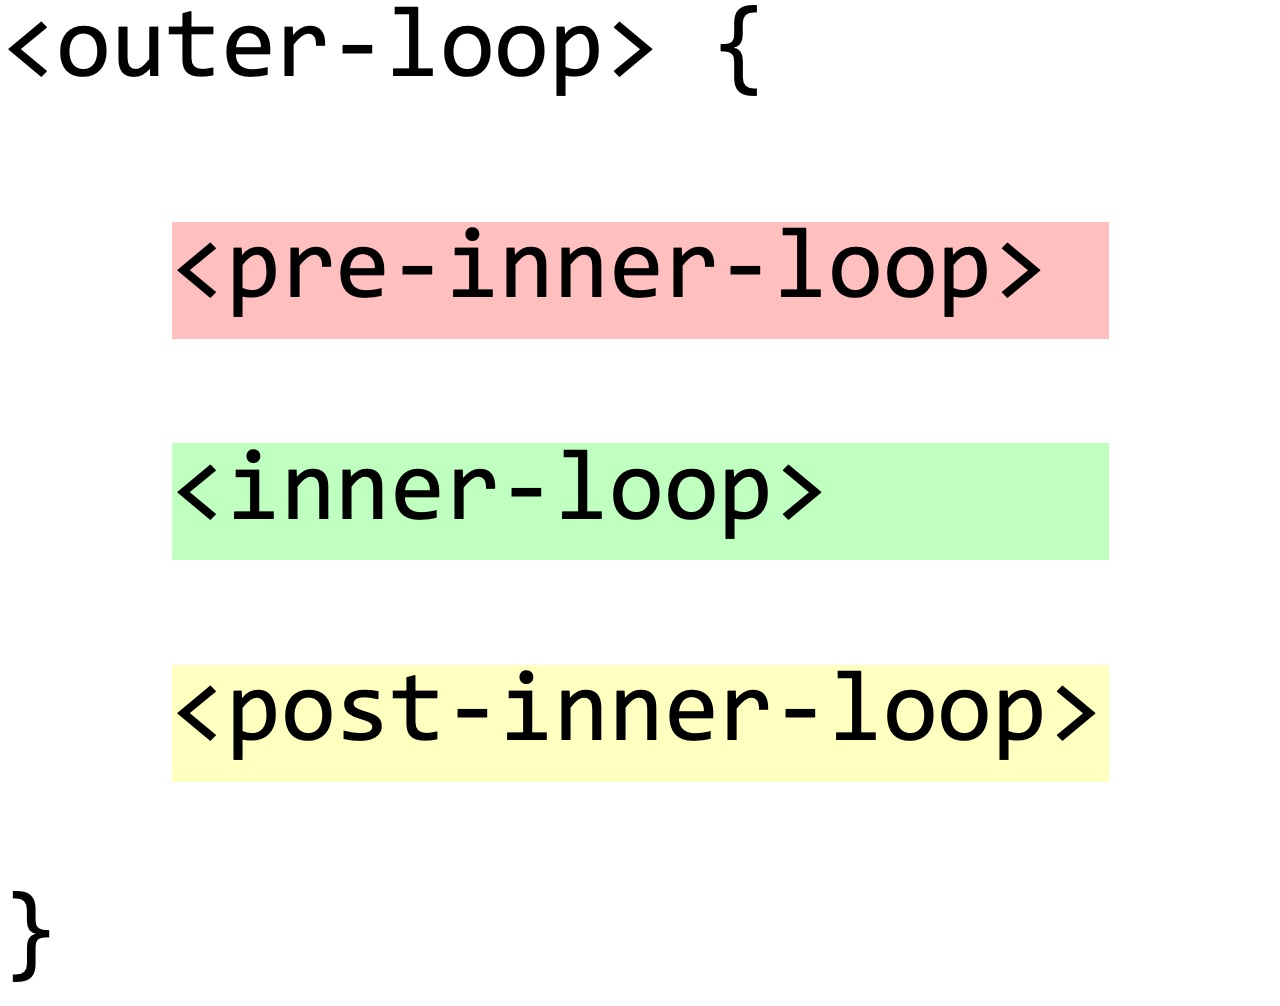
\includegraphics[width=0.6\textwidth]{embedded-loops/segment-for-loop-thinning.jpg}
    \caption{\label{fig:segment-for-loop-thinning} Sectioning of loop body statements
    for `loop thinning' process.
    Each section receives different treatment during the `loop thinning' process.}
\end{figure}
For the sake of argument, the body of the outer loop is
divided into three sections---\emph{pre-inner-loop} section, \emph{inner-loop} section, and
\emph{post-inner-loop} section---depending on their relative position
in respect to the inner loop (shown in ~\autoref{fig:segment-for-loop-thinning}).


The gist for flattening nested loops is as follows.
First, we need to move pre-loop statements out of the way.
To that end, use `loop rotation' technique (see ~\fullref{ch:loops}) backward
to unwind the pre-loop statements.
%Then internalizing the condition of inner loop so that it becomes an unconditional loop, if not
%already---for example,
%by converting the loop condition as a conditional \code{break} statement inside the loop body;
The second step depends on the inner loop construct.
If the inner loop has a \emph{non-trivial loop condition}, then the inner loop can
be converted to a conditional construct as-is by keyword swapping: \code{while} $\rightarrow$
\code{if}.
At the same time, the post-inner-loop statements shall be wrapped away in a piggybacking
\code{else}-clause.
On the contrary, if the inner loop is \emph{unconditional}, chances are that
there is a conditional \code{break} statement somewhere in the loop body.
Then one can tuck the post-inner-loop statements under the conditional of the
\code{break} statement replacing the latter, and the inner loop can be stripped away.


%shield post-loop statements in a conditional clause, probably in the `\code{else}-block' of the
%to-be-formed conditionals of next step;
%shield the post-loop statements in an additional conditional block.
%convert the inner loop---if it is an unconditional, infinite loop, just remove it, if with a
%condition, convert it to a conditional or prepend to an existing one
Throughout the process, please pay special attention to bypassing statements, such as
\code{break} and \code{continue}.
Regardless the venue taken, new conditional statements are inevitably formed.
one may refer to ~\fullref{ch:cascif} for best practices on how to organize effective
cascading conditionals.
%Note that the order of the last two steps, creating the conditional and creating the
%\code{else}-clause, may be adjusted depending on the situation---it is essentially a
%`chicken or the egg' problem.


Apart from the prescribed steps, some preparatory measures may be taken beforehand
to reduce the friction during the refactor process.
Where needed, compound statements may be taken apart before one wades deep.
Compound statements may get in your way of refactoring for multiple reasons.
The most obvious reason is that, well, parts of a compound statement
may end up at different places after refactoring.
Non-idempotent conditional expressions, such as \code{if (--i < 0)}, are even more lethal
because each execution of the condition ratchets the state of the loop, leaving no time for
taking a breath.
For example,
\begin{lstlisting}
    while (++i < LIMIT);
\end{lstlisting}
shall be expanded to
\lstinputlisting[]{embedded-loops/expanded-do-while.java}
before the start of loop thinning refactor.
The following Golang statement should also be unfolded beforehand:
\begin{lstlisting}
    if v := a[i]; v < LIMIT
\end{lstlisting}


For similar reasons, \code{for}-loop with all its header statements, should be taken apart and
converted to \code{while}-loop.
\code{while}-loop readily lends itself for `loop thinning' process, as one can
simply replace the keyword \code{while} with \code{if} at the proper time.


After `loop thinning',
aftermath changes may be performed for cleanup, convention conformation, or cosmetics.
Most importantly, following the removal of nested loops, other optimizations may become
accessible to further optimizations.
Like `Candy Crush Saga' game at a critical point, a single move may unlock a
gainful chain of reactivce moves.
This `avalanche effect' is the true value of the `loop thinning' technique.


Also note the application restrictions of the `loop thinning' process---inner loop must be directly
embedded in
outer loop with no intermediate layers;
also no bypassing statements, such as \code{break}, shall be in the pre-inner-loop section.


Most of the methods we present in this chapter are empirical, I cannot claim
universal applicability for many of them.
Instead, the techniques shall be considered on a case by case basis.
In what follows, we are going to demonstrate application of `loop thinning' technique through
a few examples adapted from real-world programming projects.


\section{Case Study: `Maximum Rectangular Area in Histogram'}
\label{sec:nested-loop-histogram}

As the first case study, let us finish a leftover project from ~\fullref{ch:loops}.
In producing the implementation as shown in snippet ~\autoref{lst:histogram-oneMoreCycle},
we removed duplicate post-loop processing code.
But the solution still looks overly complicated and messy.
What's wrong with it?
Nested loops!
Because of the nested loops, the code looks more crowded and sumptuous than it need be.
In this example, we are going to take the `loop thinning' technique for a road test.
We are going to follow closely the steps prescribed in `loop thinning' to coalesce the
nesting loops into a single loop.
The first preparatory step, converting the \code{for}-loop into a \code{while}-loop, is
straightforward and eventless.
Secondly, since there is no pre-inner-loop section, we can proceed directly with the next
step---eliminating inner loop.
To that end, we can simply replace keyword ~`\code{while}' with ~`\code{if}', using the loop
condition as is for the conditional construct.
Finally, an \code{else}-clause may be appended to the newly formed conditional statement to
house the \emph{post-inner-loop} statements, both \code{stack.push(i)} and \code{++i}, in it.
After all these are completed, the code looks like
\lstinputlisting[label={lst:histogram-coalesced-loop},
caption={Code for solving the `Maximum rectangular area under histogram' using a single loop.}]
{embedded-loops/histogram.java}


In comparison with ~\autoref{lst:histogram-oneMoreCycle}, solution in
~\autoref{lst:histogram-coalesced-loop} is much simpler and more transparent.
At a glance, one can unambiguously see its $O(N)$ runtime---for there is only one loop,
in each iteration an item is either pushed in or popped out,
and each item is subject to such operation no more than once.


Some nonessential changes may be made to make the code more compact.
For example, one may combine the two statements in the \code{else}-block into
`\code{stack.push(i++)}'.
Further, there is another category of changes that deal with excessive boundary checking,
such as
`\code{stack.isEmpty()}' and `\code{i == heights.length}'.
We will leave this to ~\fullref{ch:sentinels}.
But remember that these latter changes are optional
as they are nonessential for the `loop thinning' technique.


\section{Case Study: quicksort}\label{sec:nested-loop-quick-sort}

We will now consider another case study.
This is a classical example that was detailed by books such as `Programming
Pearls' and `Numerical Recipes'\cite{Bentley:1986:PP, NumericalRecipes:1992}.
My encounter with the code in these books completely redefined the word `simplicity'
in my dictionary.


My first implementation of the quicksort algorithm was in C based off
the traditional ``Hoare's partitioning'' scheme, as presented
in `Numerical Recipes' (minus the sentinel part).
But in what follows, I am going to present the idea in \python.


The outline of the quicksort function is as follows.
\lstinputlisting[label={lst:QuickSortOutline},language=C,
caption={An implementation of quicksort algorithm.}]
{embedded-loops/quicksort_outline.c}
where arguments \code{s} and \code{e} are the starting (inclusive) and ending (exclusive) pointers
to the array.
`\code{part}' is a recursive function whose base case is no-op, namely,
arrays with fewer than two elements.
With a pivot element randomly chosen out of the array,
a large array is partitioned into three consecutive parts: the pivot element in the middle, a
subarray on the left, and a subarray on the right.
Then the pivot element is swapped into its final position.
After this, each of the two subarrays is subject to the same function.
So on and so forth until each subarray is reduced to the base case.
At the return of the first call of the function, the entire array is left in sorted state.


As you may have noted, we emphasise that the partitioning function divides an array into three, not
two, parts---the pivot element $p$, the partition $\leq p$, and the partition $\leq p$.
This is crucial to the convergence / termination of the function.
It may be the case that one or the other of the two partitions is empty.
But even so, please remember the partitioning scheme employed in quicksort is \emph{three-way}.


With the Hoare's partitioning scheme, a tentative implementation for the function \code{part} is as
follows.
\lstinputlisting[label={lst:nestedLoopHoareMethod},language=C,
caption={Implementation of Hoare's partition scheme for quicksort.}]
{embedded-loops/quicksort_partition_sym.c}
First, we randomly select a pivot element and swap it to the beginning of the array
(ask yourself: ``why beginning of array?
Why not end?'').
Then two pointers, \code{s} and \code{e}, starting off the opposite ends of the array,
wade toward each other.
Each of them makes stop at `out-of-place' element.
When both stop, that is when a pair of `out-of-place' elements have been discovered,
a swap is performed to bring both elements to the respective partitions they belong to.
Then the pointers are back on their way toward each other once again.
So on and so forth until they meet or cross.
At that point, the pivot element (at the beginning of the array) is swapped into its final position.
Finally, a pointer pointing to this position is returned.


The above visual description of Hoare's partitioning scheme disguises the true complexity of
implementing it.
%unexpectedly tricky to implement.
so much so that once in a while when my memory of any previous implementations becomes blurry or
totally fades away, it may take me quite a few days to implement a solution that can pass a
handful of unwitty test cases.
Thus repeated several times, I decided to summary the frequently-made bugs and produced a list of
`gotcha' as follows:
\begin{enumerate}
    %    \item Pointers come to a stall before meet or cross
    \item In pivot election, failure to swap pivot element to the beginning of array
    \item For the pointers \code{s} and \code{e}, there are two hesitating options:
    `check-then-increment' or `increment-then-check'.
    The first option leads to infinite loop for certain cases.
    \item Also a choice between `\code{<= pivot}' and `\code{< pivot}' for \code{s},
    `\code{>= pivot}' and `\code{> pivot}' for \code{e}.
    Incorrect choice may inadvertently cause pointer incrementation to be skipped under
    obscure circumstances which will, in turn, cause infinite loop
    (Remember that under no circumstances, should either pointer stops approaching each other in
    any outer loop iteration before they meet or cross.)
    \item\label{itm:quicksort-boundary-condition} In the second inner loop for pointer \code{e},
    failing to check boundary condition causes `out-of-boundary' exception.
    Incorrect boundary condition, such as \code{s < e}, again cause pointer \code{e} to stall
    in the middle of the right partition.
    This will cause the pivot is placed at the wrong place at the return of function.
    \item Outer loop termination logic also needs deliberation.
    The key decision to make is `where to break or return' rather than `when to break or return'.
    For ~\autoref{lst:nestedLoopHoareMethod}, the choice of location of return
    at the end of the loop body was made after quick a few failed attempts.
    \item Fail to swap the pivot element to its final position.
    This step often poses a stumbling block for beginners as well as other unsuspecting
    developers.
\end{enumerate}
In fact just to debug ~\autoref{itm:quicksort-boundary-condition} and
figure out the correct condition \code{pivot < e}, instead of \code{s < e}, took me $2$ good hours.
Also, deciding out the semantics of the function arguments in `\code{qsort}' took me
quite some deliberation before I finally got them right.


A large part of the complication of the problem comes from the fact that this implementation
consists of many parts that are highly entangled---changing one would necessitate simultaneously
changing others.
For example,
%the return value of the partition function is picked among .
suppose we are going to change the semantics of \code{e} from exclusive to inclusive, what
would the pointer to be returned change to?
\code{s}? \code{s+1}? \code{e}? Or \code{e-1}?
Accompanying these changes, the recursive calls
\begin{lstlisting}
    qSort(s, p);
    qSort(p + 1, e);
\end{lstlisting}
also need changes.
With the choice of return value, should the recursive calls be changed to
\begin{lstlisting}
    qsort(s, p - 1)
    qsort(p + 1, e)
\end{lstlisting}
or
\begin{lstlisting}
    qsort(s, p + 1);
    qsort(p + 2, e);
\end{lstlisting}
or some other form?
The number of combinations for such changes grows exponentially as the degree of coupling increases.


This partially explains why it is so hard to correctly implement this seemingly simple partitioning
function.
On the one hand, the problem itself is complicated---the number of loose parts exceeds what our
brain can comfortably handle at once.
On the other, however, the way we approach the problem makes it harder---it is all because
we attempted to fight too many wars all at once.
The complexity of the problem is doubled, or tripled, the moment we decide to send one pointer
from each end of the array to meet somewhere in the middle.


Is there a more straightforward way to implement the quicksort algorithm?
Yes!
There is a simpler and more compact partition scheme credited to Nico Lomuto\cite{Bentley:1986:PP}.
By sending two pointers off the same end of the array, the Lomuto's partitioning scheme
successfully avoids fighting two frontiers at the same time and thus greatly simplifies the
partitioning process.


The two pointers each has a distinct task, each on its own pace.
The one running in front, so-named `frontier', is responsible to discover out-of-place elements.
The one running behind, aka, `guardian', guards the partition boundary.
When the frontier discovers an out-of-place element, the guardian pointer is incremented to make
room for it and a swap places it there.
Finally, the pivot element is swapped at the boundary place.
Notably, implementing this partitioning scheme only needs one loop
(see blow ~\autoref{lst:singleLoopLomuto}).
\lstinputlisting[label={lst:singleLoopLomuto},language=C,
caption={Implementation of Lomuto's partition scheme for quicksort.}]
{embedded-loops/quicksort_partition_asym.c}


Comparing ~\autoref{lst:nestedLoopHoareMethod} with ~\autoref{lst:nestedLoopHoareMethod},
one can't help but be surprised ``Seriously?
A single loop can replace three?''


Unlike the arduous implementation and debugging process of Hoare's,
that of the Lumoto's partitioning scheme has fewer moving parts, contains fewer surprises, and is
easier to follow.
However there is no free lunch.
The simplicity of Lumoto's quicksort comes with performance penalty
for certain cases, with one such case being large arrays with a significant amount of elements
of the same value.
In such cases,
the Lomuto's quicksort scheme tends to degrade to quadratic runtime complexity.
(Can you figure out why?)
In comparison, the Hoare's partitioning scheme is stable and
robust with respect to such cases, always performs at a steady O( N log N) expected runtime.
%\footnote{The reason is as follows.
%When faced with equal-valued elements, both ~\autoref{lst:nestedLoopHoareMethod}
%and ~\autoref{lst:singleLoopLomuto} still do pair-wise swap among two equal elements.
%But the ending position for the pivot element is seriously off to the right end of the array for
%Lomuto's partitioning scheme whereas that of the Hoare's ends up at the middle.}.
For this reason, Lomuto's partitioning scheme is not suitable for general-purpose libraries.


However, Lomuto's quicksort algorithm is still inspiring for its simplicity and elegance.
It is tempting to ask: ``Is there a quicksort implementation that has the simplicity of Lomuto's
\emph{and} the performance of Hoare's?''
I don't know for sure.
But with our `loop thinning' technique and other tools we developed in the last chapter and this, we
can explore a little bit to see if we can approach the above goal any closer than the existing
two schemes.
%Now that we have the `loop thinning' technique in hand, we can take on this challenge for a good
%cause.
%The aforementioned loop thinning technique can be used to further simplify the Hoare's partitioning
%algorithm.
Our starting point is the Hoare's quicksort implementation of ~\autoref{lst:nestedLoopHoareMethod}.
As mentioned earlier, the trickiest part of that program is the nested loops which also consists
of the major complication.
Let us forcus on getting rid of that.
%a single-loop with cascade conditionals in the loop body
%(refer to ~\autoref{ch:conditional-cascade}).


The immediate difficulty is how to take apart the densely packed conditional construct:
\begin{lstlisting}
    while(s < e && *++s < *pivot);
    while(pivot < e && *--e > *pivot);
\end{lstlisting}
The loop conditions here are unusual and awkward to handle
because both `\code{++s}' and `\code{--e}' ruthlessly ratchet the loop state forward
whenever control is passed to this line.
Namely, each evaluation of the loop condition, even if the condition evaluates to false, the
pointers `\code{s}' and `\code{e}' are still incremented.
If we use these conditions as is in the to-be conditional constructs, we would end up in a
dilemma---when we discover out-of-place elements, we would pass them without swap in the next
iteration because the program does not leave us any chance for that.


With the existing programming languages' syntaxes, we have no choice but to break
up the pre-incremental statements.
So something must be done to unfold the extraordinary loop conditions to
ordinary ones before we proceed with the rest of the `loop thinning' procedure.
As we learned in ~\fullref{ch:loops}, these loops may be converted first to
`\code{do-while} loops' such as
\lstinputlisting[language=C]{embedded-loops/quicksort_inner_loop_do_while.c}
and the latter are, in turn, converted to `\code{while} loops':
\lstinputlisting[language=C]{embedded-loops/quicksort_inner_loop_while.c}
After these changes are applied, our the partition function becomes
\lstinputlisting[language=C]{embedded-loops/quicksort_partition_sym_expanded_inner_loop.c}
You may have noticed that we have floated ~\code{--e} up in front of the first inner loop,
and this does not affect the correctness as can be verified.
The solution now seems equally messy, if not more so, as we started.
However, as you will see, this form will prove useful for the subsequent refactor step---`loop
rotation'.


Now we can proceed with the next step
of loop thinning---move the \emph{pre-inner-loop statements} out of the way.
(``Loop rotation'' is specified in ~\fullref{sec:LoopDesignConsideration}.)
After this step, the code becomes:
\lstinputlisting[language=C]{embedded-loops/quicksort_partition_sym_rotated_inner_loop.c}
We have accelerated the process by tucking the \emph{post-inner-loop statements}
resulted from the loop rotation to a conditional block.


Now we are ready with the third and most exciting step---converting inner loops to conditionals.
Now we encounter a complication that is new to us: we need to covert the second loop to an
`\code{else if}' clause of the first because the second inner loop is executed only after the first
exits.
Our final result is posted below after the conversion to conditional construct:
\lstinputlisting[label={lst:singleLoopHoarePart},language=C,escapechar=$,
caption={Implementation of partition function for Quicksort using one pointer.}]
{embedded-loops/quicksort_partition_single_loop.c}
Note that we have combined multiple statements into a compound one `~\code{swap(s++, e--)}'.
%By now we conclude our ``loop thinning' refactor process.


By now,
we achieved our goal of a quicksort partitioning implementation that has the simplicity of
Lomuto's and the robust performance of Hoare's.
In retrospection, we set off to test the hypothetical quest for a simple but performant
partitioning scheme that comprises the advantages of Lomuto's and Hoare's partitioning scheme.
Comparing with where we started off ~\autoref{lst:nestedLoopHoareMethod},
we implemented the Hoare's algorithm with a single loop plus
cascading conditionals as ~\autoref{lst:singleLoopHoarePart}.
In the process, we used the `loop rotation' techniques, the `loop thinning' techniques,
and skills concerning the construction of cascading conditionals from earlier chapters.
The new quicksort implementation retains the optimal runtime as Hoare's algorithm but has
comparable simplicity as that of Lomuto's.
That's almost too good to be true!
%If this does not impress you, then you have no feeling.
While we can make the solution simpler with the use of sentinel, we will leave that discussion to
next chapter.
However there is one change that can provide a little more saving.
If we change the semantic of ending pointer \code{e} from exclusive to inclusive, the
pre-increment before the loop (line~\ref{quicksort:pre-increment} of
~\autoref{lst:singleLoopHoarePart}) would be unnecessary.


As a byproduct of going through the detailed refactor
processes for the cases of this chapter, I want the reader to have a feeling about software
development model.
As we can see the most fruitful software development model, undoubtedly, is to come up with a
working solution first.
However shabby, messy, primitive a solution it may be, as long as it can pass a handful of unit
tests, it will be a great starting point.


Then through meticulous optimization process, for which many of the techniques we have talked
about and will be talking may be an aid, strive for straightforwardness, simplicity, and elegance.
In the course, one may discover new issues, adding new unit tests accordingly, and obtain new
solutions.
With the variety of solutions passing the same unit tests, one can often form a better
perspective regarding the solution space.
This will help one pick the most effective solution to the original problem.
%This is as a general programming guideline as well as specific  ally applicable to loops.


%\section{Case Study: Skyline Problem}\label{sec:nested-loop-skyline}
%
%%\label{Evernote:Calculate the silhouette or skyline of a group of rectangles on the horizon}
%\lstinputlisting[label={lst:silhouette-skyline},
%caption={Loop thinning example for skyline calculation.}]
%{embedded-loops/silhouette.py}
%
%\label{Evernote:Server peak load problem}
%\label{Evernote:for-loop Loop compactification examples}



%
%\section{Case Study: IV}\label{sec:nested-loop-numeral-conversion-roman}
%
%\begin{clisting}
%    \lstinputlisting[label={lst:nestedForLoop},
%    caption={Code snippet with thinned for loops.}]{embedded-loops/int_to_roman_nested_loop.java}
%\end{clisting}
%\begin{clisting}
%    \lstinputlisting[label={lst:nestedForLoop},
%    caption={Code snippet with thinned for loops.}]{embedded-loops/int_to_roman_thinned_loop.java}
%\end{clisting}


\section{Case Study: ``Needle in Haystack'' Problem}\label{sec:nested-loop-pattern-matching}

In this case study, let us consider the `needle in a haystack' problem:
\begin{quote}
``Given two strings \code{needle} and \code{haystack}, search for the first occurrence of
\code{needle} in the \code{haystack}.''
\end{quote}
String matching algorithms come with various run time complexities.
There are simple string matching algorithms with quadratic runtime complexity.
There are also fairly sophisticated algorithms that enjoy `$O(M + N)$' linear runtime,
such as Boyer-Moore algorithm
\footnote{\url{https://en.wikipedia.org/wiki/Boyer-Moore_string-search_algorithm}} and
Knuth-Morris-Pratt algorithm
\footnote{\url{https://en.wikipedia.org/wiki/Knuth-Morris-Pratt_algorithm}}.


In this section, we are going to focus on
a rudimentary, naïve algorithm with a $O(MN)$ runtime with the following considerations.
%The reasons are two-fold.
For one, this algorithm is the foundation of the more advanced algorithms.
For two, this algorithm also takes considerable coding skill to be implemented correctly.
Thus it makes a great example to illustrate
the various coding techniques we have presented so far.


The naïve algorithm is outlined as follows.
\begin{alisting}
\caption{\label{alg:string-search-naive-algorithm}
A naïve algorithm for string search whose runtime complexity is $O(MN)$ where $M$ and $N$ are
the string lengths.}
\begin{enumerate}
\item For each index \code{i} in $[0, M-1]$, the index for the character array of
the `\code{haystack}'
\begin{enumerate}
\item For each index \code{j} in $[0, N-1]$, the index for the
character array of the `\code{needle}'
\begin{enumerate}
\item If characters at \code{i} and \code{j} do not match, break the inner loop
\end{enumerate}
\item If substring \code{s[i:i+j]} equals `\code{needle}', return \code{i}
\end{enumerate}
\item return -1
\end{enumerate}
\end{alisting}


Let us begin with a nested loop solution implemented in \java as follows:
\begin{clisting}
\lstinputlisting[label={lst:nestedLoop-string-search},caption={Code snippet with nested loops.}]
{embedded-loops/pattern_match_nested_loop.java}
\end{clisting}
We make this our starting point because it is the most easily thought of solution.
If this problem appears in the final exam or a coding challenge for a software engineer hiring,
chances are that you will see this a lot in the submitted works.


%Note that the abortion of the inner loop upon the first pair of mismatched
%characters is
%discovered or running out of character in \code{haystack}.
Before we apply the heavy-duty code simplification techniques,
it is a low-hanging fruit resulting in immediate improvement---one can safely end the search of the
`\code{needle}' when the remaining part of the `\code{haystack}' is shorter than the `\code{needle}'.
With this change, the condition for the outer loop becomes
\begin{lstlisting}
i + needle.length() <= haystack.length()
\end{lstlisting}



An improvement on the inner loop may be to resolve the awkward scope of the loop variable
\code{j}.
Currently the scope of \code{j} has to extend beyond the inner loop because
its value is needed after the loop.
There are several options to resolve this awkwardness.
One is to use the `one-more-cycle' technique (see ~\pageref{sec:one-more-cycle} for more details).
Instead of terminating at $j = N$, let it terminate at $j = N+1$ so that the last
iteration may be dedicated to return successful search result.
If done this way, the loop condition will be unnecessary as the loop is
either aborted in an earlier iteration or terminated on the $N+1$th iteration.
With these changes, the nested loop solution is shortened:
\lstinputlisting[label={lst:nestedLoop-one-more-cycle},caption={Code snippet with nested loops.}]
{embedded-loops/pattern_match_nested_loop_one_more_cycle.java}


With the handful of code tuning, we have made the code simpler and shorter.
But that's not all
We have so far gotten rid of the most commonly made implementation kinks.
%That is about what we can do with nested loops.
Even though we achieved simplification of a few lines, that is not all.
We can simplify the implementation even further by doing away with the nested loop.


To that end, we will follow the prescriptions of `loop thinning' in
~\autoref{sec:loop-thinning-technique}.
Let us first prepare the code for the `loop thinning' process.
First off, let us convert all \code{for} loops to \code{while}-loops so as to reduce refactor
friction.
This implies that the increment statements, \code{++j} and \code{++j} are to be relocated to ends
of the corresponding loop bodies.


Then as usual, we eliminate the \emph{pre-inner-loop statements} by `loop rotation' in the
reverse sense, namely, we rotate the loop to `loosen' the program.
This will result in the statement `int j = 0' being used twice---once before the outer loop as
initialization and once at the end of the loop body to reset \code{j} to 0.
As a result, the initialization statement `\code{int j = 0}' is duplicated with one copy
at the forefront of the outer loop with the other after the last statement within the outer loop.
Also the inner loop now becomes an unconditional loop \code{while(true)}.
If you are still with me, the code now looks like this:
\lstinputlisting[escapechar=~]{embedded-loops/pattern_match_thinning_loop_intermediate_stage.java}
It is important to check and verify that this code still passes the same amount of
unit tests as ~\autoref{lst:nestedLoop-one-more-cycle} does.
This is the invariant that should be maintained at each important milestone
through a refactoring process.


Now we come to the second step of `loop thinning'.
Since the \code{break} statement in the inner loop is the only path that leads to the
execution of post-inner-loop statements, we can tuck them all under the same
conditional block wherein the \code{break} statement is.
Also, the condition for the same conditional statement is complementary to that of the
increment statement `\code{++j}', so we could shield \code{++j} in an \code{else} clause.


Hooray!
We are ready to remove the unconditional inner loop---and it is as simple as ``just strip it away''.
After this step, the code looks like this:
\lstinputlisting[]{embedded-loops/pattern_match_thinned_loop_intermediate_stage.java}
Finally as a cleanup step, the condition on line~\ref{line:haystack-needle} of the previous listing
may be absorbed into the loop condition.
Also the loop condition may be switched from
\begin{quote}
\code{i + needle.length() <= haystack.length()}
\end{quote}
to
\begin{quote}
\code{i + j < haystack.length()}
\end{quote}
The final version after this change is:
\lstinputlisting[label={lst:thinnedLoop},caption={Code snippet with nested loops.}]
{embedded-loops/pattern_match_thinned_loop.java}
without affecting correctness but made it more direct to ensure the safety of subsequent index
operation in the expression `\code{haystack.charAt(i + j)}'.

This completes the `loop thinning' process.
Looking back where we started, the latest version of implementation is both succinct and easier to
understand.


\section{Conclusion}\label{sec:loop-push-up-conclusion}

%What used to be one loop per data structure can actually be achieved with a one-layer loop plus
%cascade conditionals.


Nested loops are hard to understand and often pose obstacle to code refactor and extension.
%As can be seen, where nested loops occur are mostly related to dynamics adjustment to a
%streamlined processing code.
While compelling, many usages of nested loops can be
substituted with one simple loop and the resultant code is usually much simplified.
I strongly advise the avoidance of nested loops in production code whenever possible.


The `loop thinning' technique is a tunneling mechanism by which developers can overcome
refactor barriers to discover new and exciting implementations from known ones.
Even if the resulting solutions is not guaranteed simpler, the new solutions thus discovered often
offer valuable perspectives for inspiring better coding practices.
%Even if this is not possible or inconvenient, one can still boost the readability by
%factoring nested loops into more meaningful, reusable functions.
